\section{Background}

This section gives a reader unfamiliar with the field exactly the concepts
needed to follow the rest of the report: the ETSI NFV framework (what an NFVI
is), and the 5G core as a set of cloud-native functions (what runs \emph{on}
the NFVI). We deliberately keep it short and concrete --- only what the design
later depends on.

\subsection{The ETSI NFV framework: who provides, who consumes}

ETSI's reference architecture \cite{etsi002} separates the system into three
domains, shown in Figure~\ref{fig:etsi}.

\begin{figure}[H]
    \centering
    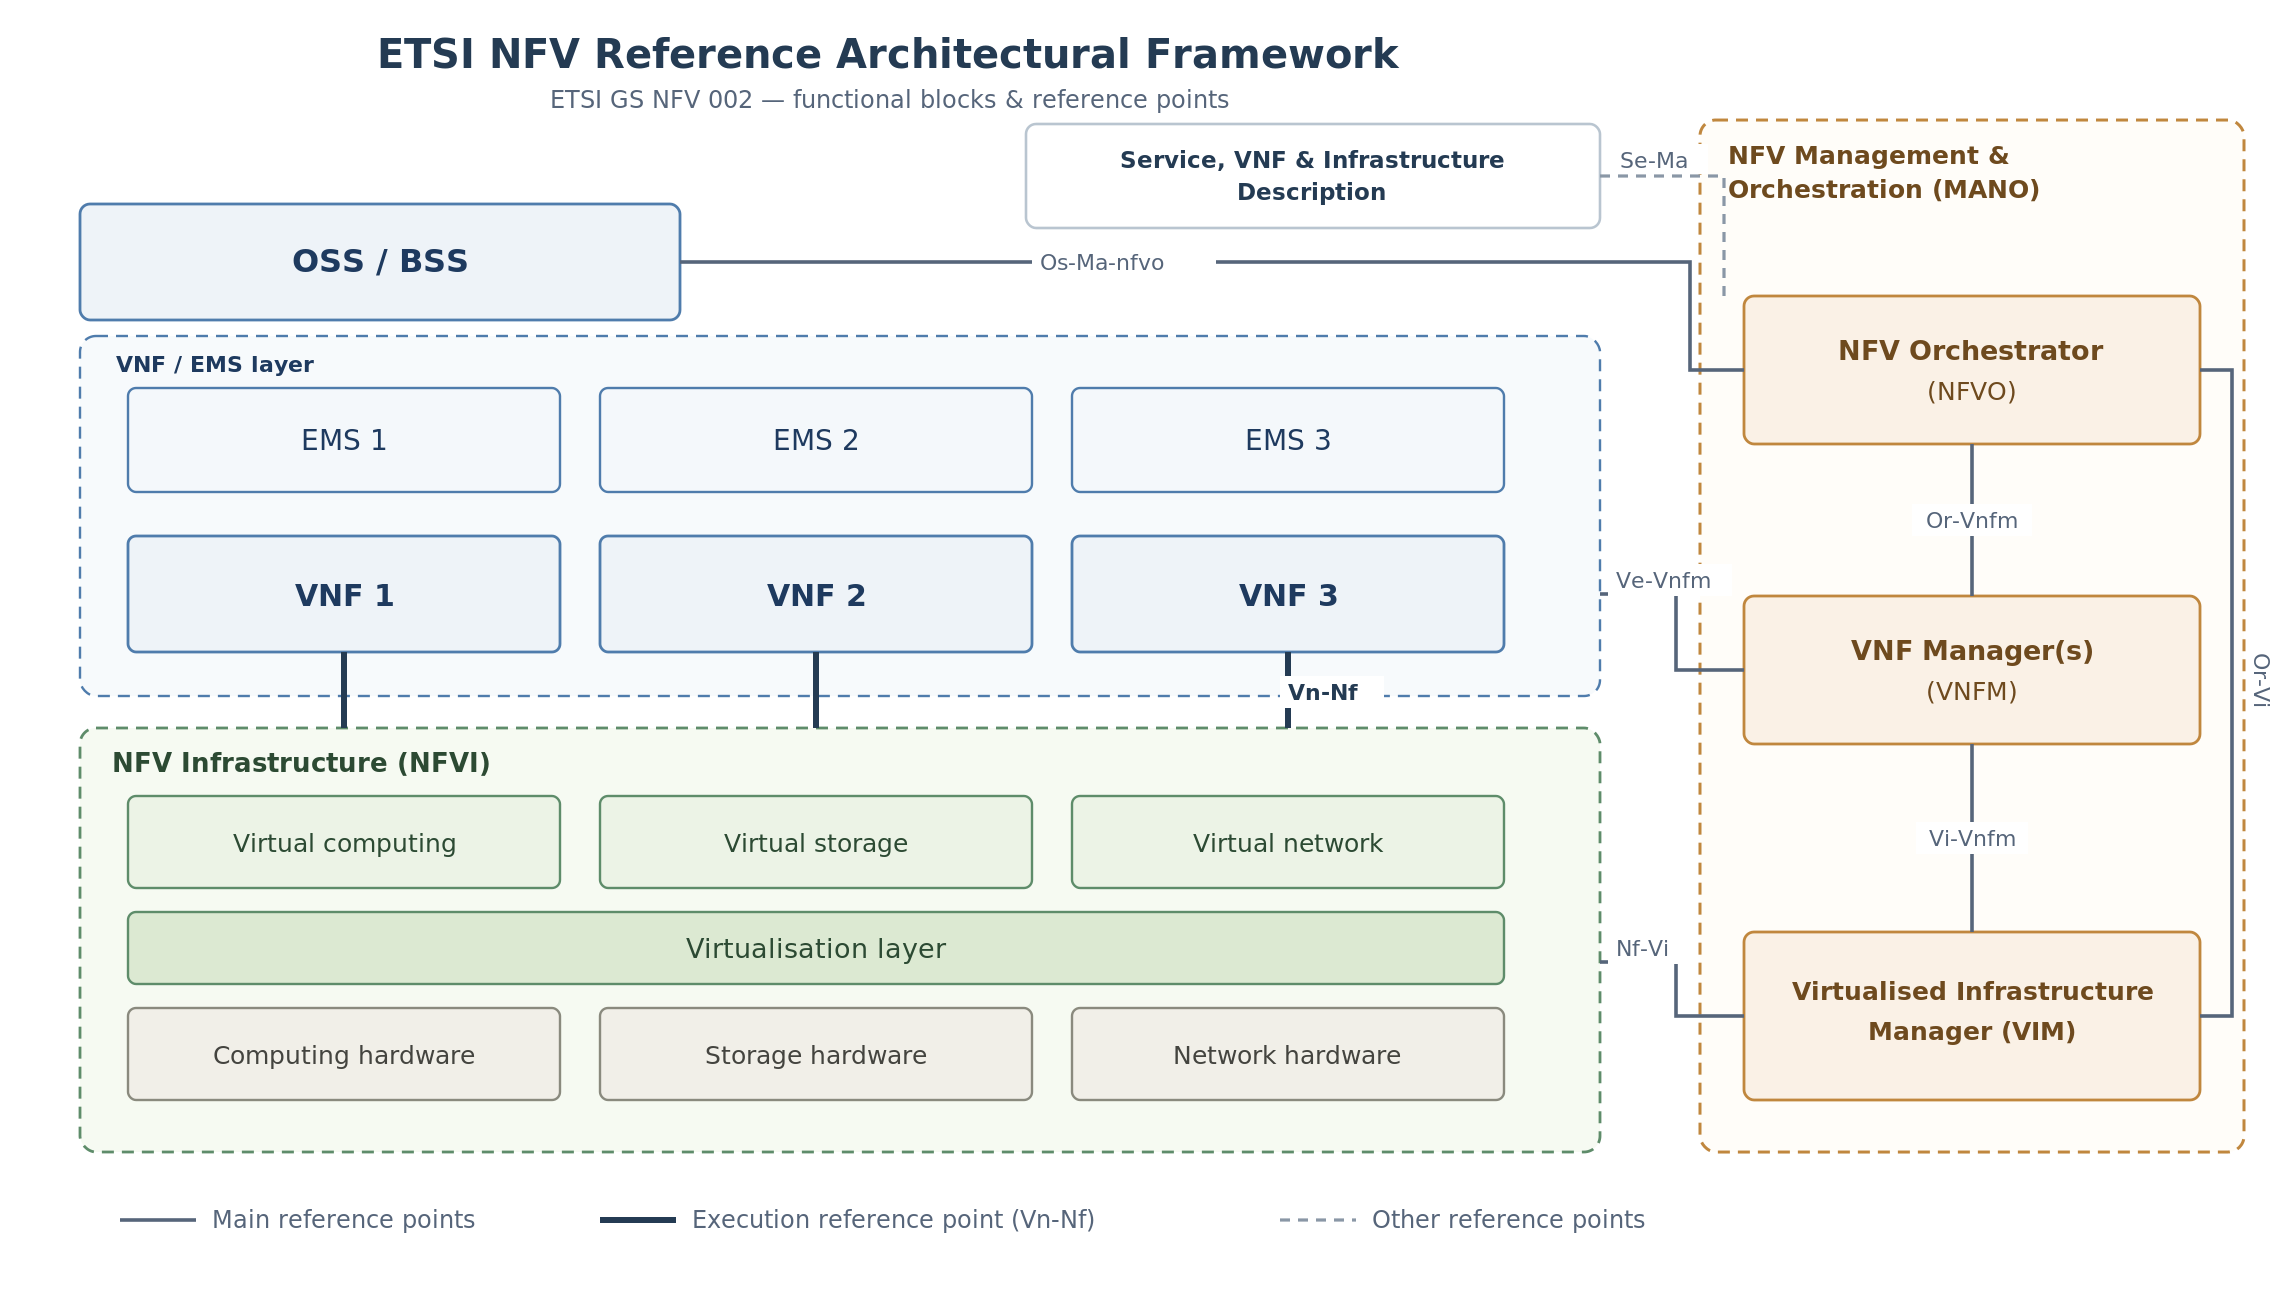
\includegraphics[width=0.9\textwidth]{Images/etsi_nfv_arch.png}
    \caption{ETSI NFV framework and how this project realises each block.}
    \label{fig:etsi}
\end{figure}

\begin{itemize}
    \item \textbf{NFVI} --- the infrastructure: compute, storage, and network,
          plus the virtualisation layer. It is the \emph{provider} of
          resources. In this project the NFVI is the three-node k3s cluster.
    \item \textbf{VNF / CNF} --- the network functions themselves, the
          \emph{consumers} of the infrastructure. Here they are the Open5GS 5G
          core functions, running as containers.
    \item \textbf{MANO} (Management and Orchestration) --- the \textbf{VIM}
          manages NFVI resources (this is Kubernetes/k3s), the \textbf{VNFM}
          manages the lifecycle of each function (here, Helm), and the
          \textbf{NFVO} orchestrates end-to-end network services.
\end{itemize}

The single most important idea is the provider/consumer split: \emph{this
project builds the provider (NFVI) and validates it with a real consumer (the
5G core).} That distinction is what was missing from a naive reading of ``a
three-node cluster''.

\subsection{The 5G Standalone core as cloud-native functions}

The 5G SA core \cite{ts23501} is decomposed into NFs that talk to each other
over a \textbf{Service-Based Interface (SBI)} --- HTTP/2 REST APIs --- much
like microservices. The functions relevant to this project are:

\begin{itemize}
    \item \textbf{AMF} --- handles UE registration and mobility; it is the
          control-plane entry point from the radio network (interface
          \textbf{N2}).
    \item \textbf{SMF} --- manages PDU sessions (a UE's data connection) and
          controls the UPF over interface \textbf{N4}.
    \item \textbf{UPF} --- the \emph{only} user-plane function: it forwards
          actual subscriber packets. It receives them from the radio side over
          \textbf{N3} (a GTP-U tunnel) and sends them to the data network over
          \textbf{N6}.
    \item \textbf{NRF} --- a registry where every NF registers and discovers
          the others; stateless and read-heavy.
    \item \textbf{AUSF, UDM, UDR, PCF, NSSF, SCP} --- supporting control-plane
          functions (authentication, subscriber data, policy, slice selection,
          and an SBI proxy). UDR keeps subscriber records in a database
          (MongoDB).
\end{itemize}

\paragraph{Control plane vs.\ user plane --- the decisive separation.}
5G makes a hard split between the \textbf{control plane} (signalling: who is
this subscriber, may they connect, set up a session) and the \textbf{user
plane} (the subscriber's actual data packets). The control NFs (AMF, SMF, NRF,
\ldots) exchange small SBI messages; the UPF moves bulk traffic at high rate.
This is why the UPF is given its own dedicated network interfaces (N3/N6) and
why, in our cluster, those interfaces must \emph{not} share the path used for
ordinary control signalling. This requirement drives the entire network design
in Section~4.

\subsection{Why Kubernetes alone is not enough}

Kubernetes is an excellent VIM, but a default pod has exactly one network
interface, attached by a single \textbf{CNI} (Container Network Interface)
plugin to one cluster-wide overlay. That suffices for web microservices, but
not for a UPF that needs separate user-plane interfaces. The gap is filled by
a \textbf{secondary CNI}: \textbf{Multus}, a meta-plugin that lets a pod be
attached to additional networks. Section~3 turns this and the other gaps into
an explicit list of requirements.

We use \textbf{k3s} \cite{k3s}, a CNCF-certified single-binary Kubernetes
distribution that replaces etcd with a lightweight embedded datastore --- ideal
for a 16~GB host while remaining fully API-compatible with upstream Kubernetes.
